\documentclass[12pt]{article}


\usepackage{amssymb}
\usepackage{amsmath}
\usepackage{fullpage}
\usepackage{epsfig}
\usepackage{epstopdf}
\everymath{\displaystyle}

\newif\ifans

\anstrue

\begin{document}

\begin{center}
\underline{\LARGE{Chapter 1.3 Practice Problems}}
\end{center}

\noindent EXPECTED SKILLS:

\begin{itemize}

\item Be able to determine limits at infinity - especially for polynomials, rational functions, functions involving radicals, exponential functions, and logarithmic functions.

\item Use algebraic techniques to help with indeterminate forms of $\displaystyle \frac{\pm\infty}{\pm\infty}$ and $\infty-\infty$.

\item Use substitutions to evaluate limits of compositions of functions.

\end{itemize}

\noindent PRACTICE PROBLEMS:

\begin{enumerate}

\item Based on the graph of $F(x)$ shown below, compute the indicated limits.  (Make reasonable assumptions about the behavior of the function outside of the shown region.)

\begin{center}
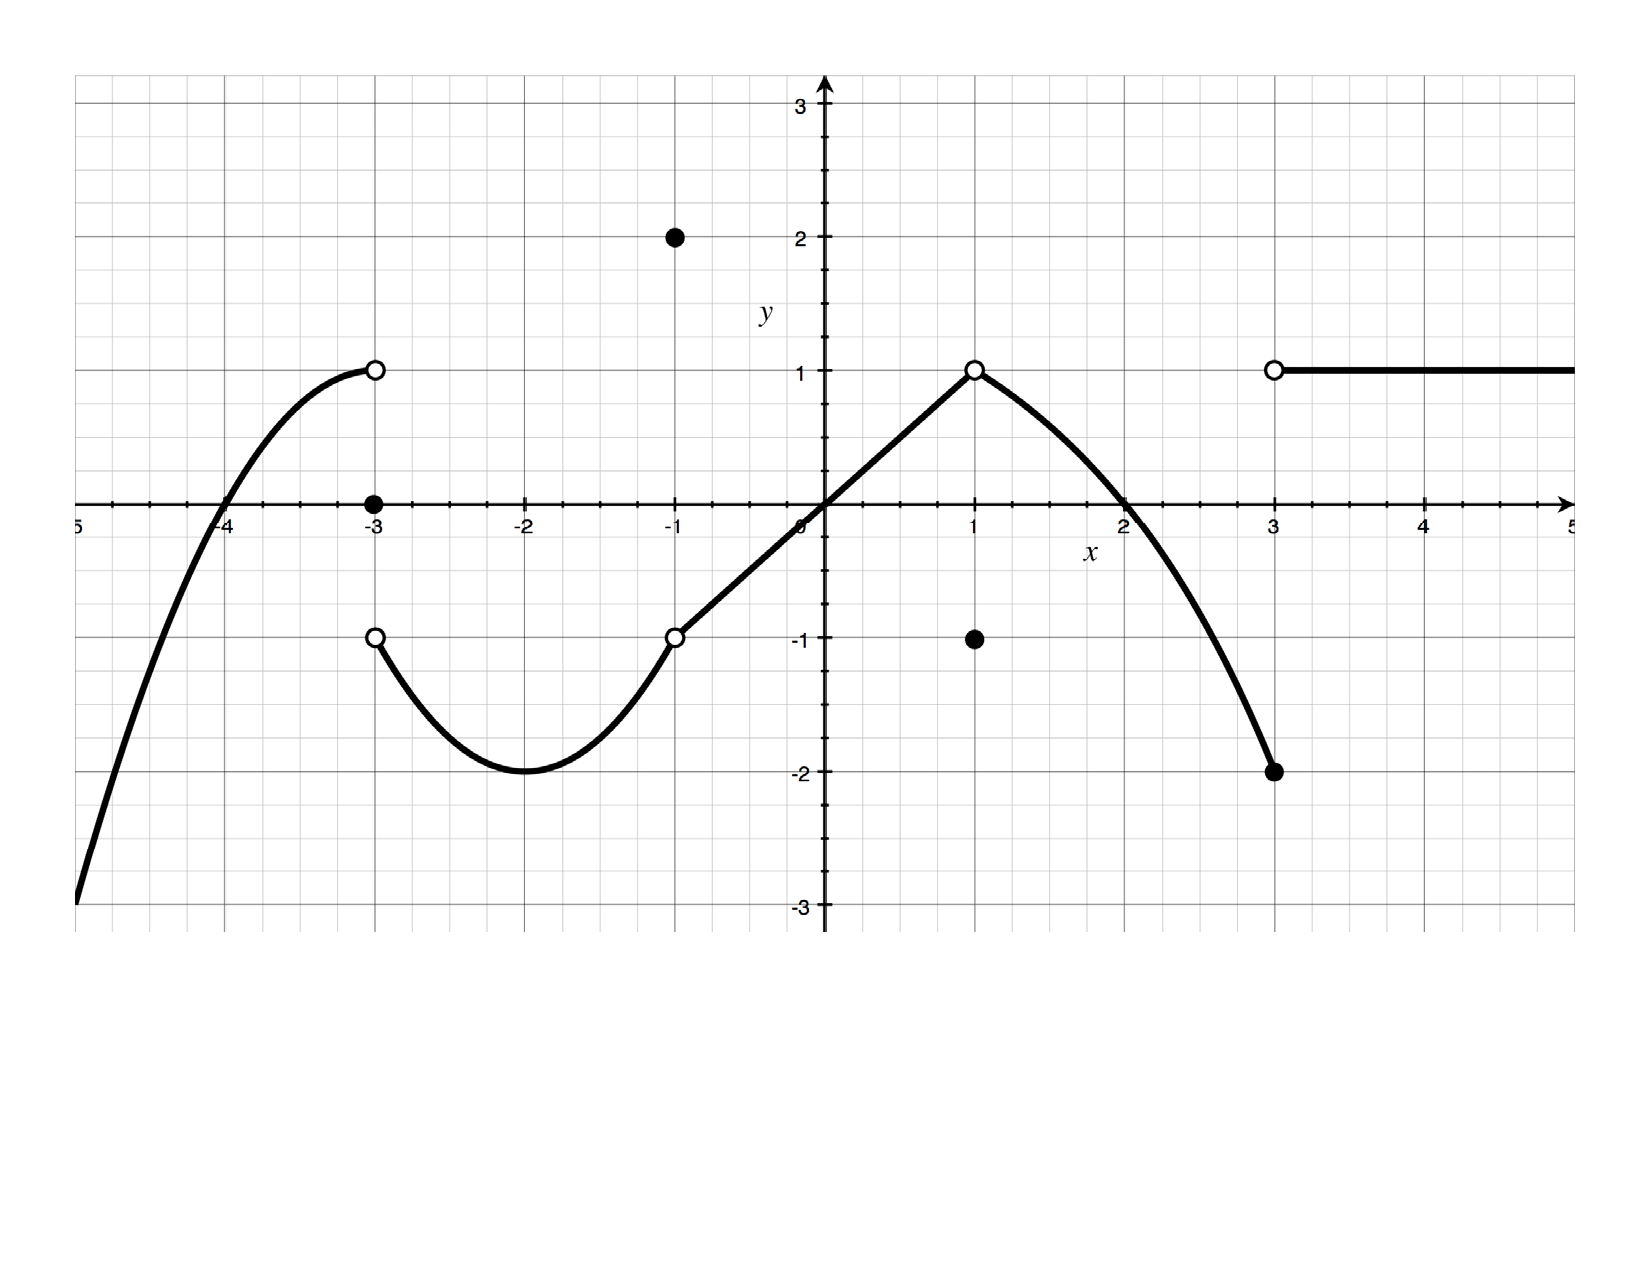
\includegraphics[scale=0.5]{Limits1.pdf}
\end{center}

\begin{enumerate}

\item $\displaystyle \lim_{x \rightarrow +\infty}{F(x)}$

\ifans{\fbox{1}} \fi

\item $\displaystyle \lim_{x \rightarrow -\infty}{F(x)}$

\ifans{\fbox{$-\infty$}} \fi

\end{enumerate}

\newpage

\item Based on the graph of $G(x)$ shown below, compute the indicated limits.  (Make reasonable assumptions about the behavior of the function outside of the shown region.)

\begin{center}
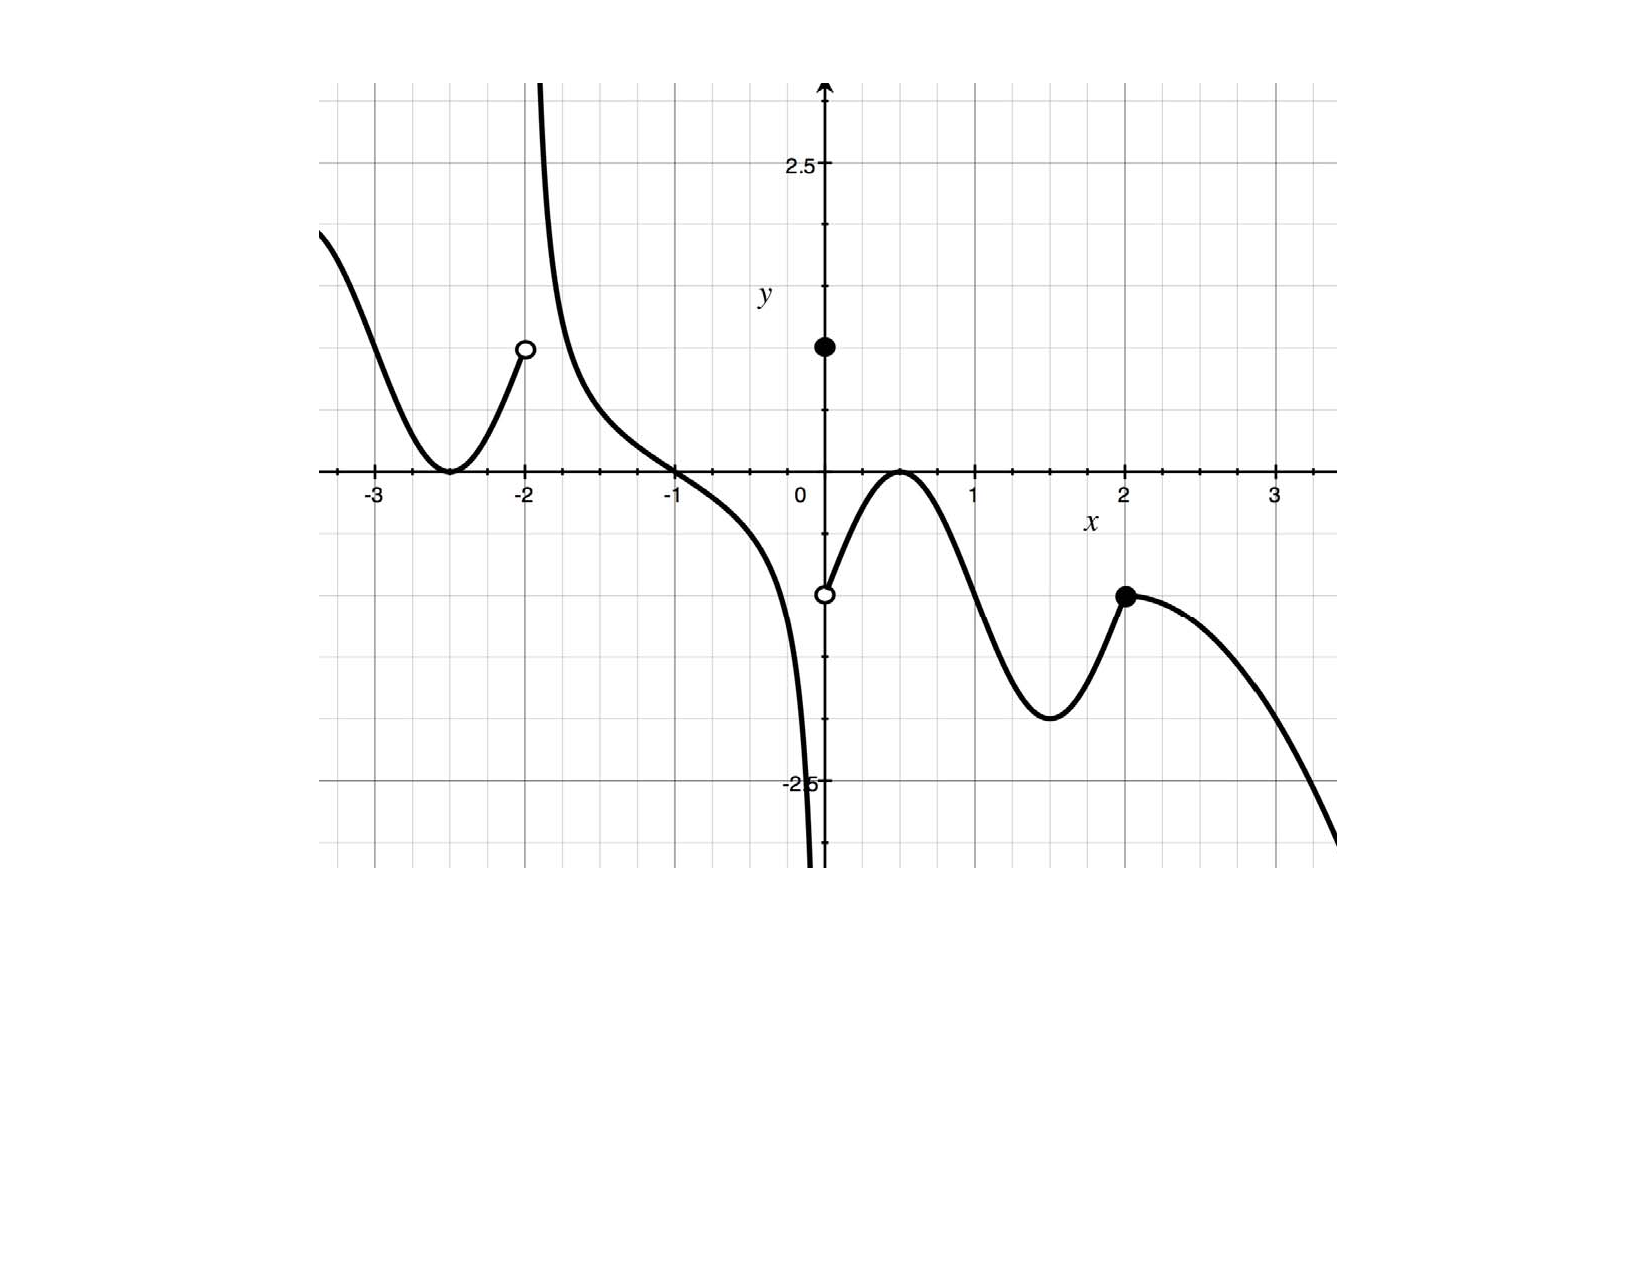
\includegraphics[scale=0.5]{Limits3.pdf}
\end{center}

\begin{enumerate}

\item $\displaystyle \lim_{x \rightarrow +\infty}{G(x)}$

\ifans{\fbox{$-\infty$}} \fi

\item $\displaystyle \lim_{x \rightarrow -\infty}{G(x)}$

\ifans{\fbox{$+\infty$}} \fi

\end{enumerate}

\end{enumerate}

\noindent {\bf For problems 3-32, compute the limit. If the limit doesn't exist write $+\infty$, $-\infty$, or DNE (whichever is most appropriate).}

\begin{enumerate}
\setcounter{enumi}{2}

\item $\displaystyle \lim_{x\rightarrow \infty}{1}$

\ifans{\fbox{1}} \fi

\item $\displaystyle \lim_{x\rightarrow \infty}{\left(x^2+1\right)}$ 

\ifans{\fbox{$+\infty$}} \fi

\item $\displaystyle \lim_{x \rightarrow \infty}{x^2(x-7)(5-x)}$

\ifans{\fbox{$-\infty$}} \fi

\item $\displaystyle \lim_{x\rightarrow \infty}{\left(5-\frac{1}{x}+\frac{4}{x^3}\right)}$

\ifans{\fbox{5}} \fi

\item $\displaystyle \lim_{x\rightarrow -\infty}{\left(\frac{300}{x^{200}}\right)}$

\ifans{\fbox{0}} \fi

\item  $\displaystyle \lim_{x\rightarrow \infty}{\left(\frac{3x+2}{x}\right)}$ 

\ifans{\fbox{3}} \fi

\item  $\displaystyle \lim_{x\rightarrow \infty}{\left(\frac{-x+3}{x^2}\right)}$

\ifans{\fbox{0}} \fi

\item  $\displaystyle \lim_{x\rightarrow \infty}{\left(\frac{x^2}{x-1}\right)}$

\ifans{\fbox{$+\infty$}} \fi

\item  $\displaystyle \lim_{x\rightarrow \infty}{\left(\frac{3x^5-4x}{2x^5-4x^3-4x+5}\right)}$

\ifans{\fbox{$\displaystyle \frac{3}{2}$}} \fi

\item  $\displaystyle \lim_{x\rightarrow \infty}{\left(\frac{x^4-3x^2+5}{100x^3-10}\right)}$

\ifans{\fbox{$+\infty$}} \fi

\item  $\displaystyle \lim_{x\rightarrow -\infty}{\left(\frac{x^2-4x+6}{9-x}\right)}$

\ifans{\fbox{$+\infty$}} \fi

\item  $\displaystyle \lim_{x\rightarrow -\infty}{\left(\frac{x^3-12x+12}{x+10}\right)}$

\ifans{\fbox{$+\infty$}} \fi

\item $\displaystyle \lim_{x \rightarrow \infty}{\left(\frac{\sqrt{4+3x^2}}{2+2x}\right)}$
%Webwork

\ifans{\fbox{$\displaystyle \frac{\sqrt{3}}{2}$}} \fi

\item $\displaystyle \lim_{x \rightarrow -\infty}{\left(\frac{\sqrt{4+3x^2}}{2+2x}\right)}$
%Webwork

\ifans{\fbox{$\displaystyle -\frac{\sqrt{3}}{2}$}} \fi

\item $\displaystyle \lim_{x \rightarrow \infty}{\left(\frac{2x^3-5x+6}{8-9x^2-x^3}\right)}$

\ifans{\fbox{$-2$}} \fi

\item  $\displaystyle \lim_{x\rightarrow \infty}{e^{x}}$ 

\ifans{\fbox{$+\infty$}} \fi

\item  $\displaystyle \lim_{x\rightarrow -\infty}{e^x}$ 

\ifans{\fbox{0}} \fi

\item  $\displaystyle \lim_{x\rightarrow -\infty}{\left(\frac{1}{e^x}\right)}$ 

\ifans{\fbox{$+\infty$}} \fi

\item  $\displaystyle \lim_{x\rightarrow \infty} e^{1/x}$ 

\ifans{\fbox{1}} \fi

\item $\displaystyle \lim_{x \rightarrow \infty}{\left(\frac{7}{e^x-8}\right)}$

\ifans{\fbox{0}} \fi

\item $\displaystyle \lim_{x \rightarrow -\infty}{\left(\frac{7}{e^x-8}\right)}$

\ifans{\fbox{$\displaystyle -\frac{7}{8}$}} \fi

\item $\displaystyle \lim_{x\rightarrow 0^+}{\ln{x}}$ 

\ifans{\fbox{$-\infty$}} \fi

\item  $\displaystyle \lim_{x\rightarrow \infty}{\ln{x}}$ 

\ifans{\fbox{$+\infty$}} \fi

\item $\displaystyle \lim_{x\rightarrow \infty}{\left(\frac{\ln{6x}}{\ln{2x}}\right)}$

\ifans{\fbox{1}} \fi

\item $\displaystyle \lim_{x\rightarrow \infty}{\left[\ln{(x+2)}-\ln{(3x+5)}\right]}$

\ifans{\fbox{$\displaystyle \ln{\left(\frac{1}{3}\right)}$}} \fi

\item $\displaystyle \lim_{x \rightarrow \infty}{\left(\sqrt{x^2+8x-15}-x\right)}$

\ifans{\fbox{$4$}} \fi

\item $\displaystyle \lim_{x \rightarrow \infty}{\left(x+\sqrt{x^2+2x}\right)}$

\ifans{\fbox{$+\infty$}} \fi

\item $\displaystyle \lim_{x \rightarrow -\infty}{\left(x+\sqrt{x^2+2x}\right)}$

\ifans{\fbox{$-1$}} \fi

\item  $\displaystyle \lim_{x\rightarrow \infty}{\left(\sqrt{x^2-x}-x\right)}$

\ifans{\fbox{$\displaystyle -\frac{1}{2}$}} \fi

\item A tank contains 5000 liters of pure water.  Brine containing 30 grams of salt per liter of water is pumped into the tank at a rate of 25 liters per minute.  It can be shown thta the concentration of salt in the tank after $t$ minutes is:

$$C(t)=\frac{30t}{200+t}$$

What happens as $t \rightarrow \infty$?

\ifans{\fbox{The concentration of salt approaches $30$ g/L}} \fi

\end{enumerate}

\noindent {\bf Use the following two definitions to answer questions 33-36.}

\begin{itemize}

\item {\bf Definition:} A function $f(x)$ has a \underline{horizontal asymptote} of $y=L$ if at least one of the following is true:

\begin{itemize}

\item[$\circ$] $\displaystyle \lim_{x \rightarrow \infty}{f(x)}=L$

\item[$\circ$] $\displaystyle \lim_{x \rightarrow -\infty}{f(x)}=L$.

\end{itemize}

\item {\bf Definition:} A function $f(x)$ has a \underline{vertical asymptote} of $x=a$ if at least one of the following is true:

\begin{itemize}

\item[$\circ$] $\displaystyle \lim_{x \rightarrow a^-}{f(x)}=+\infty$

\item[$\circ$] $\displaystyle \lim_{x \rightarrow a^-}{f(x)}=-\infty$

\item[$\circ$] $\displaystyle \lim_{x \rightarrow a^+}{f(x)}=+\infty$

\item[$\circ$] $\displaystyle \lim_{x \rightarrow a^+}{f(x)}=-\infty$

\end{itemize}

\end{itemize}

\begin{enumerate}
\setcounter{enumi}{32}

\item Compute the equations of all horizontal asymptotes and vertical asymptotes, if any, for each of the following functions.

\begin{enumerate}

\item $\displaystyle f(x)=\frac{4x}{x-3}$

\ifans{\fbox{Vertical Asymptote: $x=3$, Horizontal Asymptote: $y=4$}} \fi

\item $\displaystyle f(x)=\frac{x^2-5x+4}{x^2-6x+8}$

\ifans{\fbox{Vertical Asymptote: $x=2$, Horizontal Asymptote: $y=1$}} \fi

\end{enumerate}

\item Let $y=f(x)$ satisfy the following:

\begin{itemize}

\item $\displaystyle \lim_{x\rightarrow \infty}{f(x)}=\infty$

\item $\displaystyle \lim_{x\rightarrow -\infty}{f(x)}=-7$

\item $\displaystyle \lim_{x\rightarrow 6^+}{f(x)}=\infty$

\item $\displaystyle \lim_{x\rightarrow 6^-}{f(x)}=-\infty$

\end{itemize}

Based on this information, determine equations for the horizontal and vertical asymptotes of $f(x)$.

\ifans{\fbox{Vertical Asymptote: $x=6$; Horizontal Asymptote: $y=-7$}} \fi

\item Sketch a function $y=f(x)$ which satisfies the following conditions. (There are many possible answers.)

\begin{itemize}

\item $f(2)=0$

\item $\displaystyle \lim_{x \rightarrow \infty}{f(x)}=\lim_{x \rightarrow -\infty}{f(x)}=0$

\item $\displaystyle \lim_{x \rightarrow -3^-}{f(x)}=\infty$

\item $\displaystyle \lim_{x \rightarrow -3^+}{f(x)}=-\infty$

\item $\displaystyle \lim_{x \rightarrow 0}{f(x)}=-\infty$

\end{itemize}

\ifans{\fbox{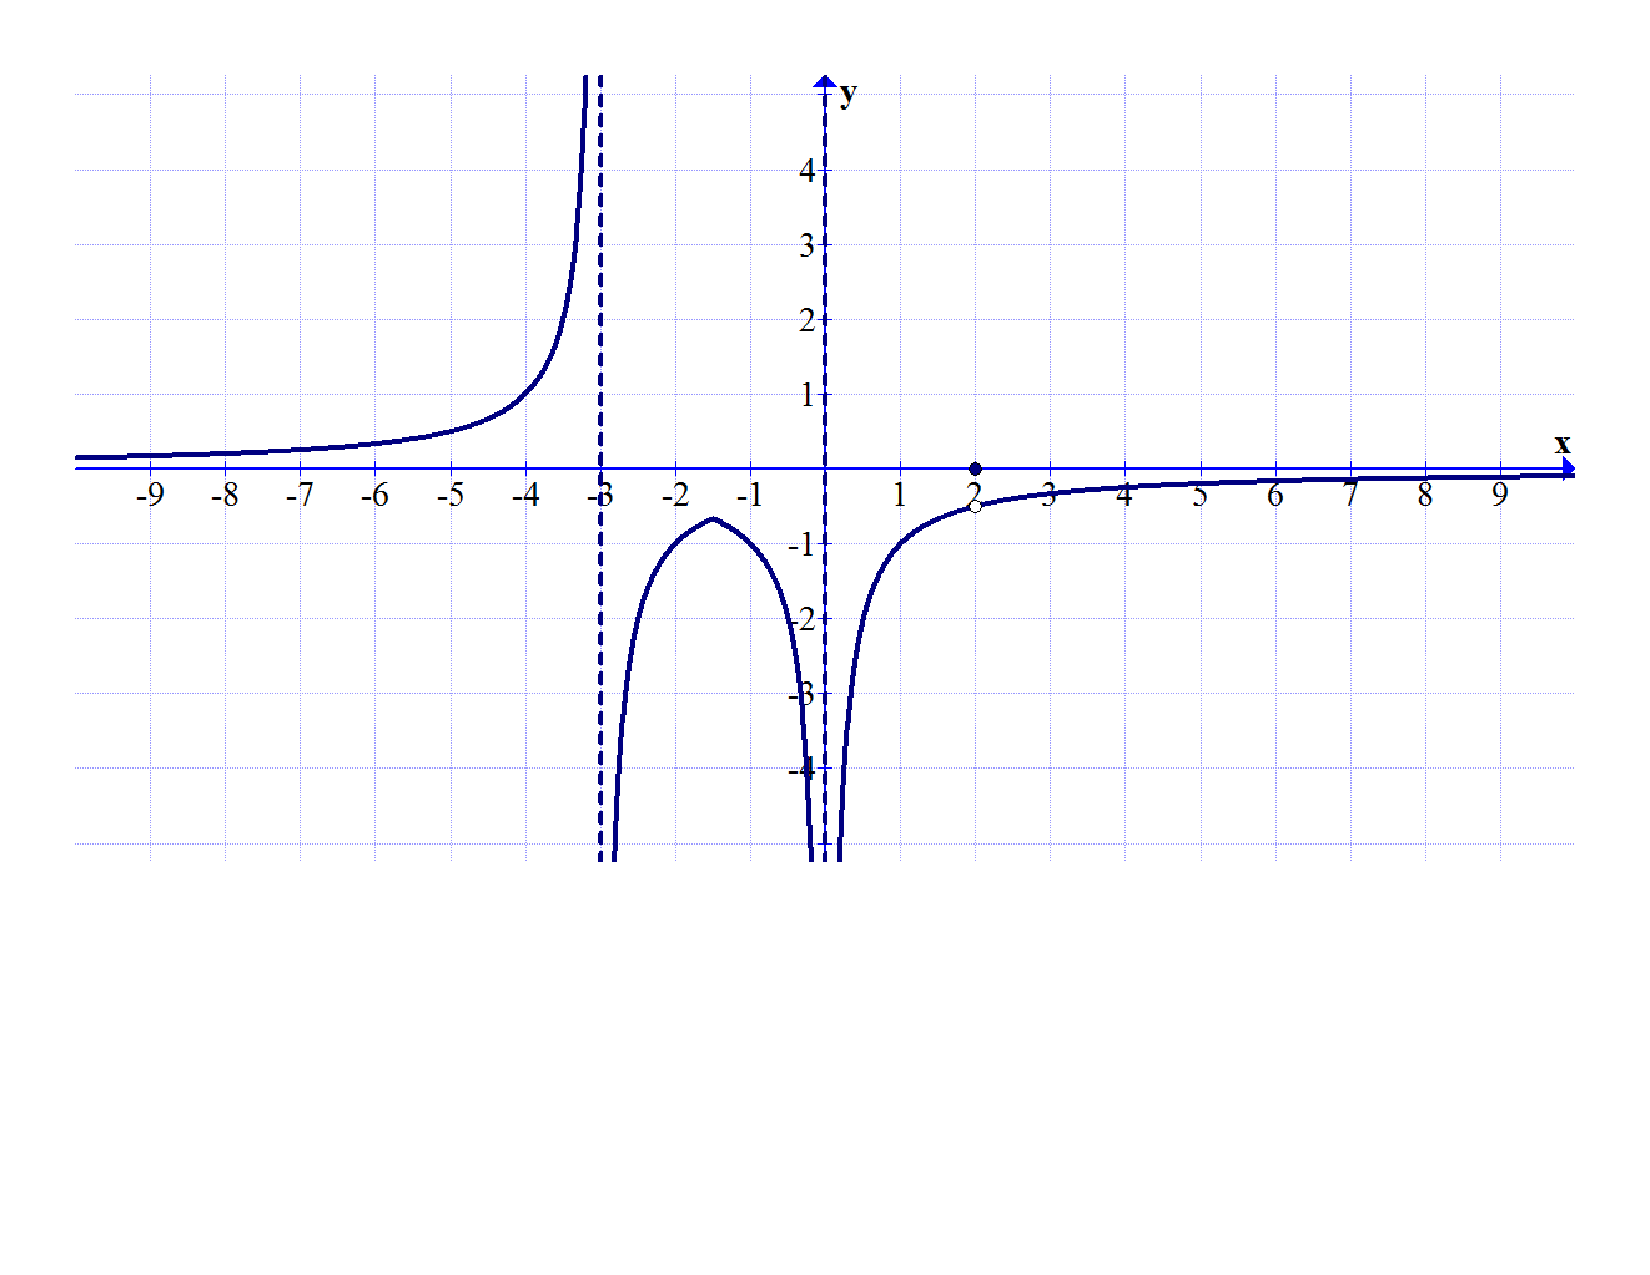
\includegraphics[scale=0.5]{graph.pdf}}} \fi

\item Determine whether the following statement is true or false.  If the statement is true, explain why.  If the statement is false, provide a specific counterexample.

\begin{center}
\emph{``A function $y=f(x)$ can have at most two horizontal asymptotes."}
\end{center}

\ifans{\fbox{\parbox{1\linewidth}{True.  We determine the horizontal asymptotes of $y=f(x)$ by computing the end behavior; i.e., we compute $\lim_{x\rightarrow +\infty}f(x)$ and $\lim_{x\rightarrow -\infty}f(x)$.  Having a finite value for either of these limits will yield a horizontal asymptote.  So, if $\lim_{x\rightarrow +\infty}f(x)=L$ and $\lim_{x\rightarrow -\infty}f(x)=M$ (where $L$ and $M$ are distinct, finite, real numbers), then $f(x)$ has two horizontal asymptotes $y=L$ and $y=M$.  For a specific example of a function with two horizontal asymptotes, consider $f(x)=\tan^{-1}(x)$.}}} \fi

\item Consider $f(x)=x^2+1$.

\begin{enumerate}

\item Estimate the area between the graph of $f(x)$ and the $x$-axis on the interval $[0,6]$ using 2 rectangles of equal width and right endpoints, as in the diagram below.  Is your estimate an overestimate or an underestimate of the actual area?

\begin{center}
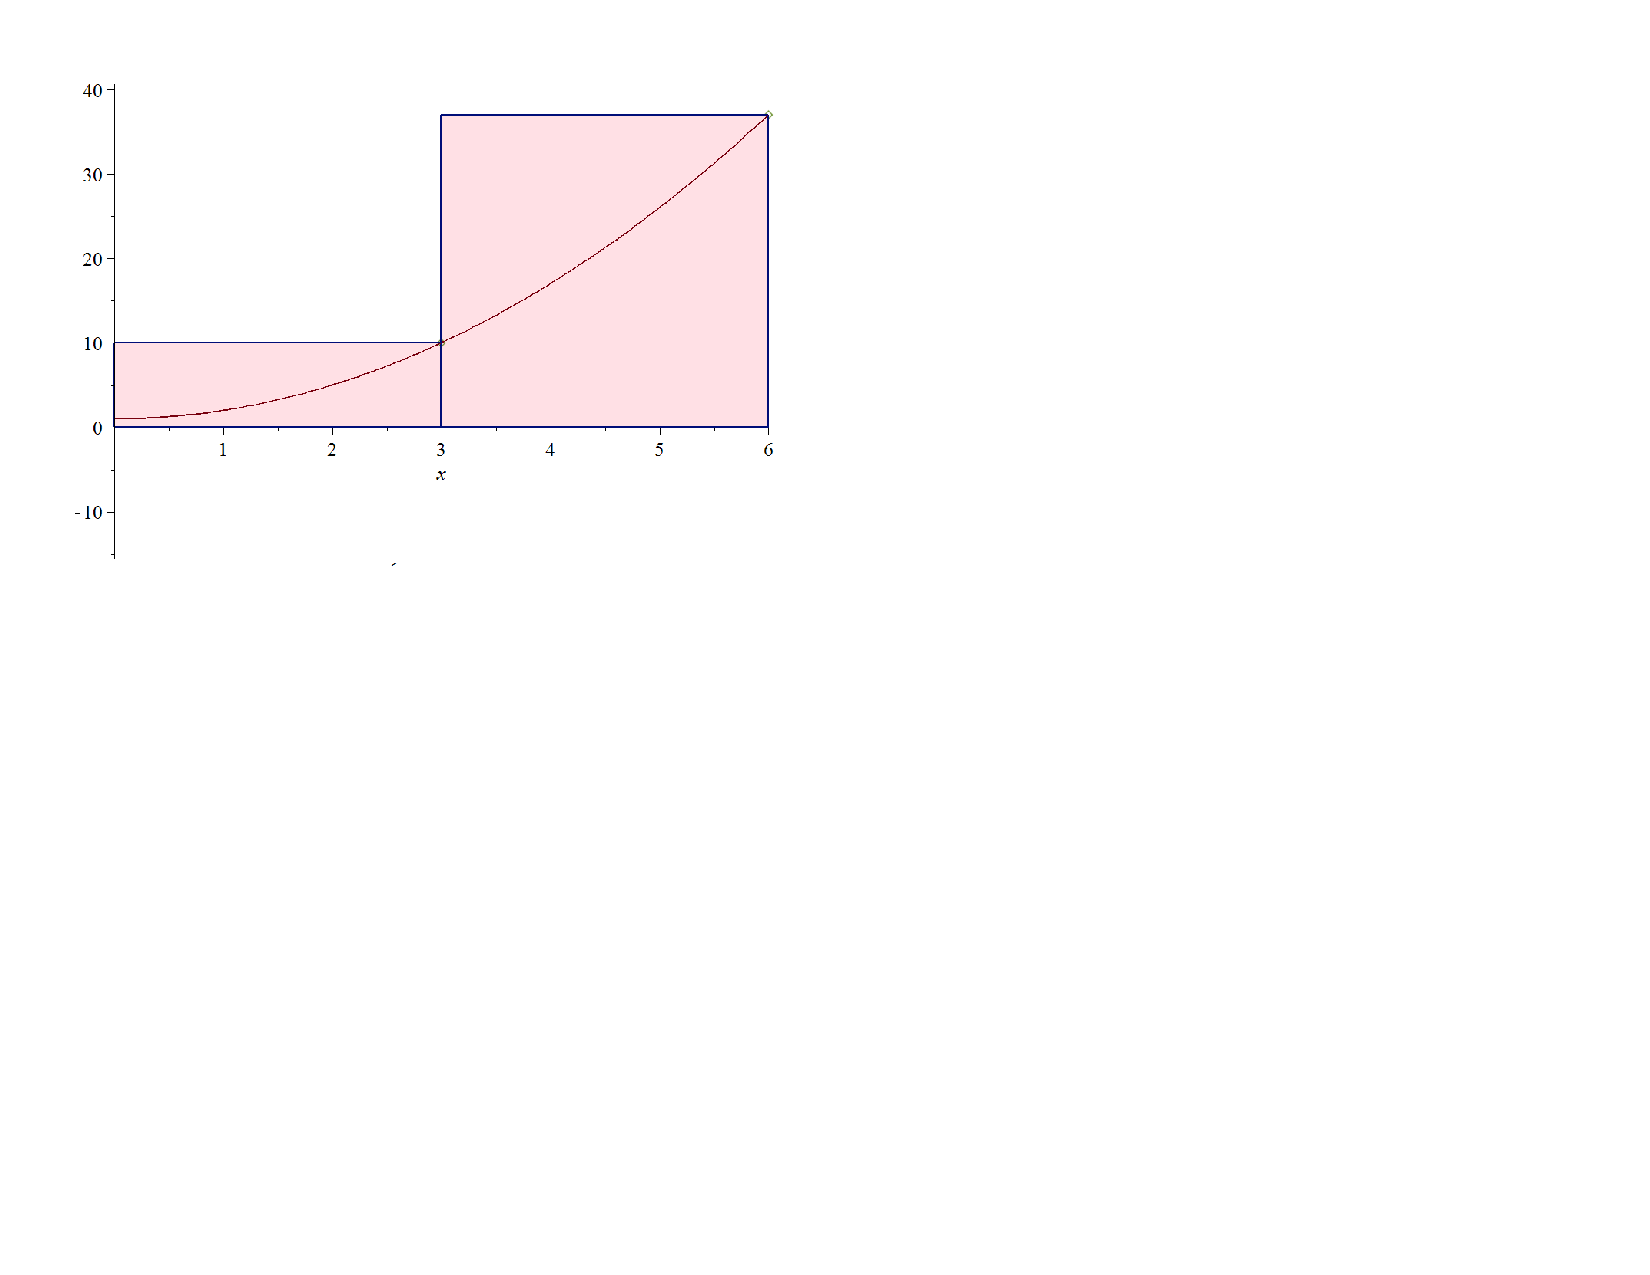
\includegraphics[scale=0.5]{2rect.pdf}
\end{center}

\ifans{\fbox{$A\approx 141$; This is an overestimate.}} \fi

\item Estimate the area between the graph of $f(x)$ and the $x$-axis on the interval $[0,6]$ using 3 rectangles of equal width and right endpoints, as in the diagram below.  Is your estimate an overestimate or an underestimate of the actual area?  How does this estimate compare to your estimate from part (a)?

\begin{center}
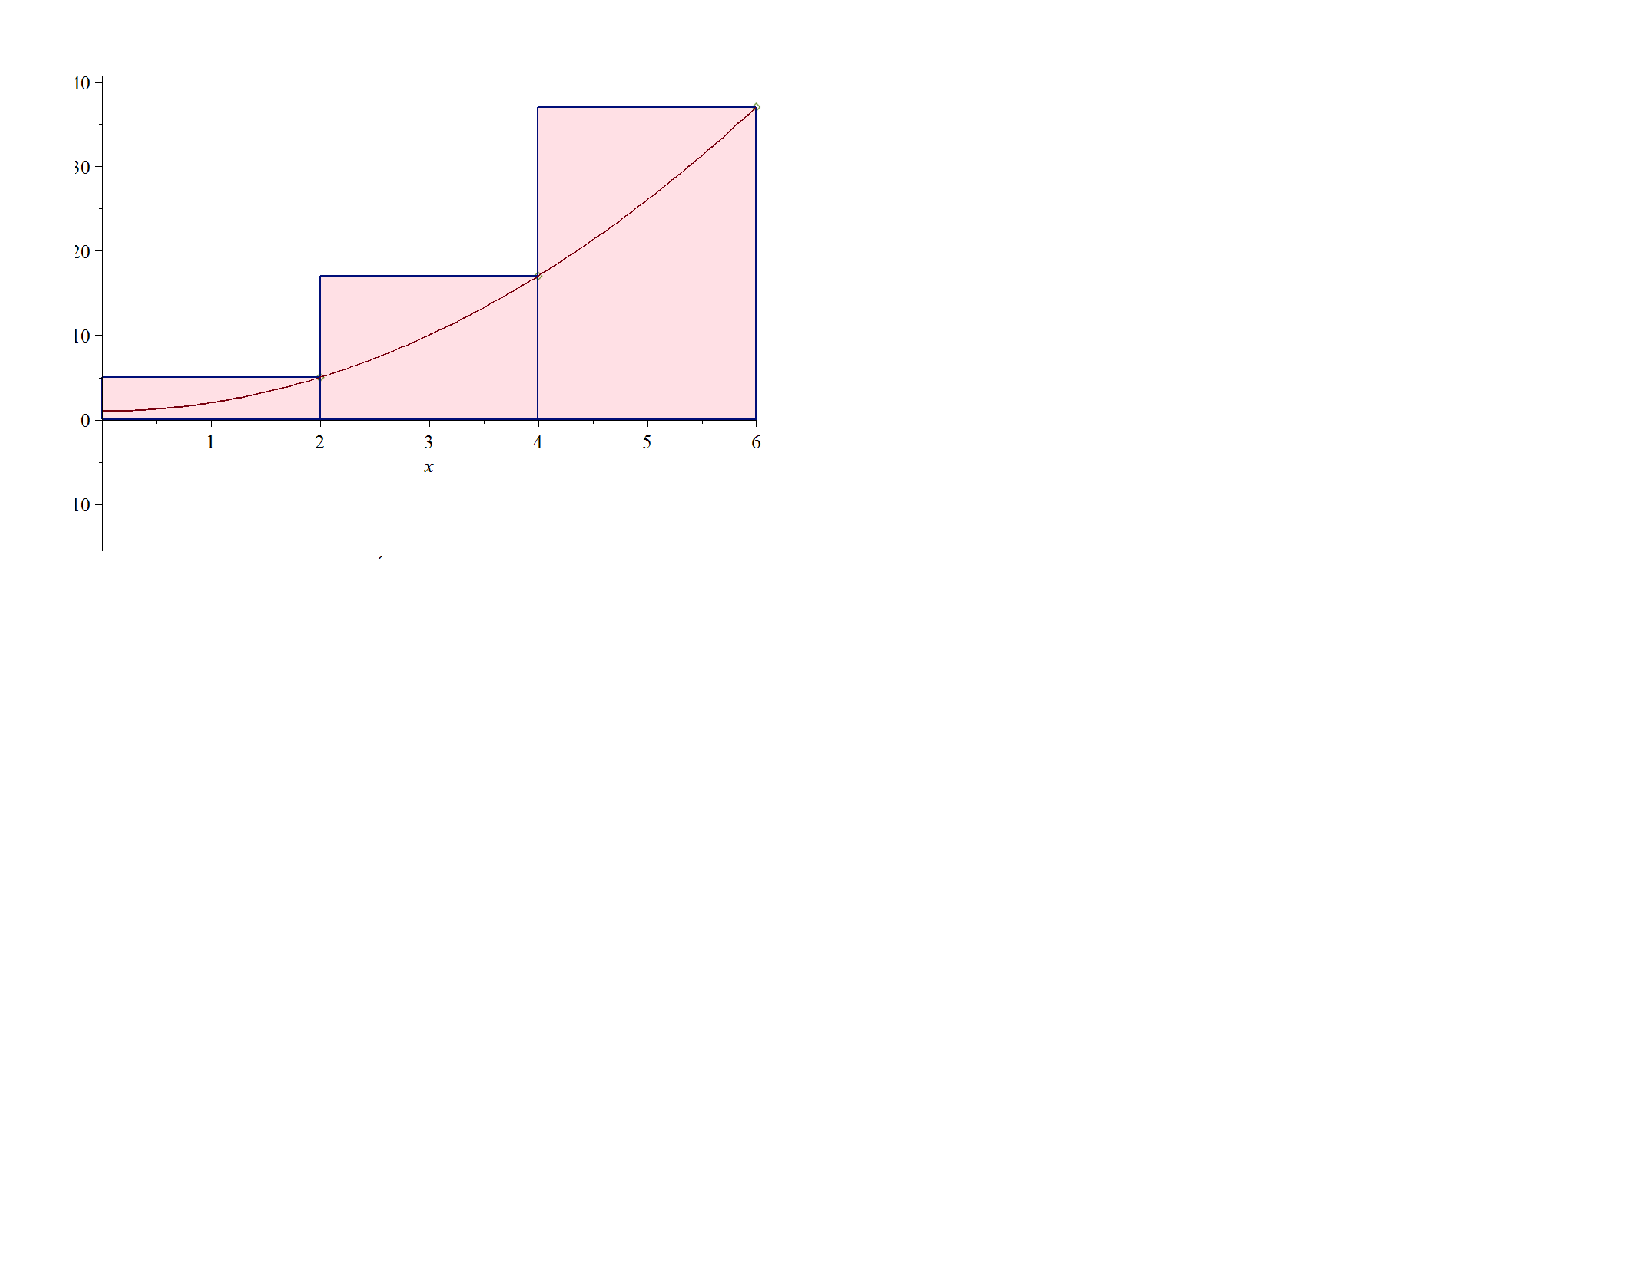
\includegraphics[scale=0.5]{3rect.pdf}
\end{center}

\ifans{\fbox{\parbox{1\linewidth}{$A\approx 118$; This is an overestimate; but, it is closer to the actual area than the estmate from part (a).}}} \fi

\item It can be shown that an estimate of the area between the graph of $f(x)$ and the $x$-axis on the interval $[0,6]$ using $n$ rectangles of equal width and right endpoints can be expressed as $A(n)=\frac{36(n+1)(2n+1)}{n^2}+6$.  Compute $\lim_{n\rightarrow +\infty}A(n)$ and interpret your answer.

\begin{center}
Depicted below are $n=30$ rectangles\\
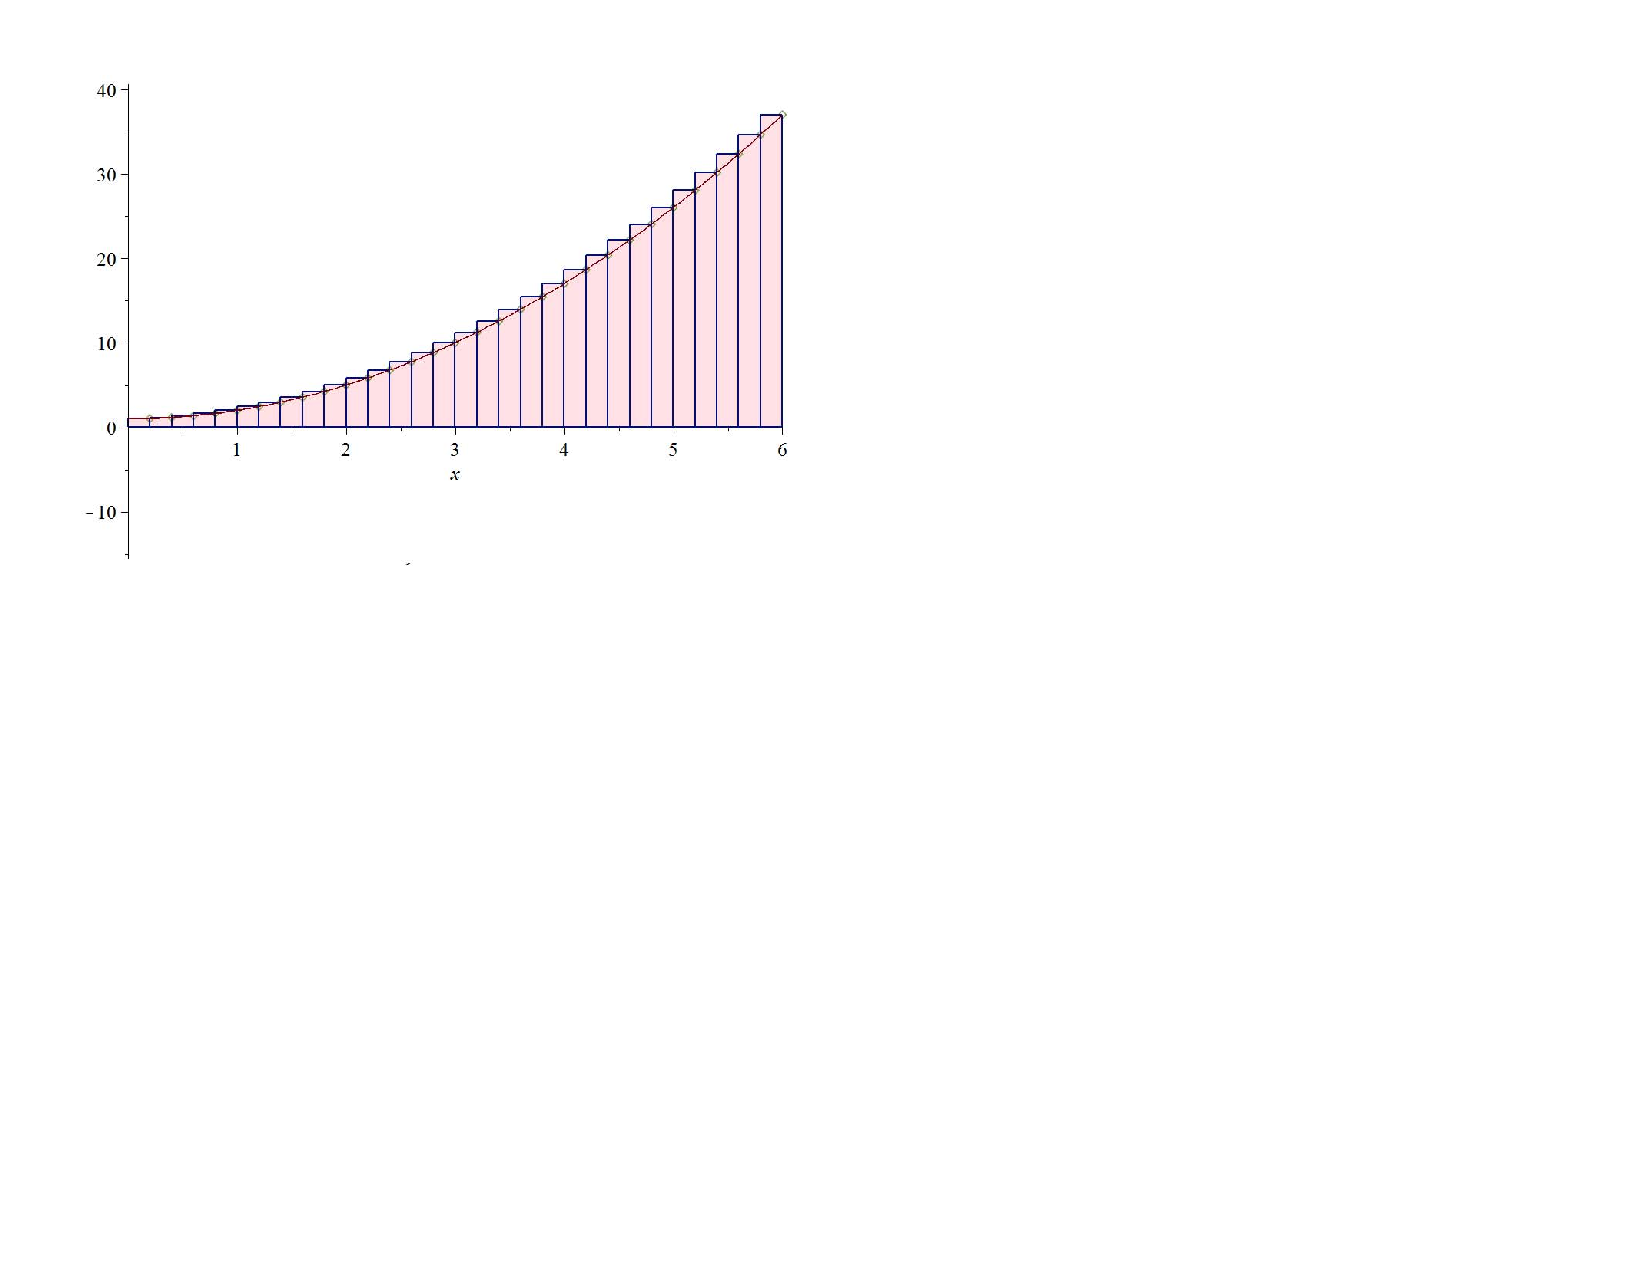
\includegraphics[scale=0.5]{nrect.pdf}
\end{center}

\ifans{\fbox{$\lim_{n\rightarrow +\infty}A(n)=78$.  This is the exact area between the graph of $f(x)$ and the $x$-axis on $[0,6]$}} \fi

\end{enumerate}

\end{enumerate}

\end{document}